\section{Structures discrètes sur l'internet}

\subsection{Ressources}
Livre : sur iCampus 
\begin{itemize}
\item Chapitre 1-5 (Graphe = modèle des réseaux) définitions, concepts (liens forts et faibles), contexte des réseaux, relations positives et négatives
\item Chapitre 13 (Structure du Web)
\item Chapitre 14 (Analyse des liens sur le web)
\item Chapitre 18 (Lois de puissances)
\item Chapitre 20 (Les phénomènes de petit monde)
\end{itemize}
\subsection{Exemple et analyse de graphes}
Voici quelques commentaires réalisés sur les figures du $1^{er}$ chapitre :
\begin{itemize}

	\item \textbf{Figure 1.1} (ci dessous : Figure \ref{karate} Illustration des relations amicales entre 34 personnes dans un club de karaté.
Chaque nœud représente une personne et chaque lien, un lien d'amitié entre ces personnes.
On constate que tout le monde n'est pas ami avec tout le monde. Grâce à cette structure, on peut déduire certaines choses, par exemple : deux personnes ont beaucoup de liens d'amitié avec d'autres personnes mais pas entre eux.\\
\begin{figure}[!h]
\centering
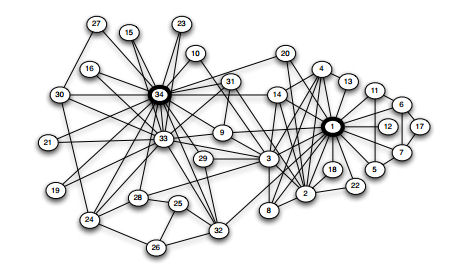
\includegraphics[scale=1]{images/17_karate_club.jpg}
\label{karate}
\caption{Relations amicales dans un club de karaté}
\end{figure}

	\item \textbf{Figure 1.2} Des employés dans un laboratoire de recherche (nœud) ont des liens entre eux :
Lignes claires = communication e-mail.
Lignes foncées = hiérarchie, organisation du laboratoire.
On voit que la communication entre les gens suit relativement bien la structure hiérarchique, mais pas complètement. On peut voir comment les gens collaborent, leurs degrés de collaboration, etc... \\

	\item \textbf{Figure 1.3} On constate que dans cette illustration, il y a beaucoup plus de nœuds. Chaque nœud est une institution financière (banque par exemple). Chaque nœud a un chemin vers un autre nœud (il y a des liens entre toutes les banques). Le centre est très dense, ça montre une faiblesse du système financier : si une banque dans le centre fait faillite par exemple, toutes les autres banques liées à elle sont également mises en danger . Donc si le noyau central est trop grand, c'est une faiblesse. En regardant cette structure, on peut trouver les faiblesses et les comprendre. Ca peut être très important.\\

	\item \textbf{Figure 1.4} Un nœud représente un blog politique et un lien, une référence vers un autre blog. Nous avons deux partis qui représentent chacun un noyau : les démocrates et les républicains. On constate qu'il y a moins de connexions entre les deux noyaux qu'à l'intérieur de ceux-ci. On peut visualiser cette structure et se poser des questions : est-ce que ce monde bipolaire est un problème ?\\\
\end{itemize}

Ce sont divers exemples que nous allons essayer d'analyser. Sur Internet, il y a beaucoup de nœuds avec de grandes capacités de calcul et de stockage. On peut maintenant regarder ces structures (pas avant). 
\subsection{Introduction}
\begin{itemize}
\item Structure des réseaux (Facebook, Twitter, réseau économique,...).
\item Comportement des participants (interactions : chaque nœud sera un participant et va interagir).En principe chaque nœud ne voit que son voisinage et interagit en conséquence.
\begin{itemize}


	\item Interactions LOCALES avec conséquence GLOBALES.
	Il faut faire le lien entre ces deux choses.
	\item Effets non attendus. Ex: réseaux routiers (nœud = automobilistes, lien = routes) : \\
	S'il y a des bouchons, on augmente la capacité du réseau (ajouter une voie par exemple)
	Le résultat peut être non intuitif, ça peut être :
	\begin{itemize} 
		\item Une réduction des transferts.
		\item Une réduction du trafic. (résultat contre celui attendu)
	\end{itemize}	
	\item Le \textbf{Paradoxe de Braess} nous dit que l'ajout d'une nouvelle capacité à un réseau peut 	réduire la performance globale (effet non attendu).
Il faut donc comprendre comment le réseau fonctionne au lieu de faire n'importe quoi et avoir des effets non attendus.
\end{itemize}
\end{itemize}
\subsection{Nouvelle discipline}
Les graphes et leurs propriétés évoluent avec le temps, ce n'est pas statique.\\
$\Rightarrow$Nouvelles disciplines pour analyser des graphes Youtube, Flicker, etc...\\
Synthèse de 3 disciplines :
\begin{enumerate}

	\item La théorie des graphes => mathématique
	\item La théorie des jeux => mathématique
		Exemple : Youtube impose ses règles et ceux qui utilisent Youtube sont des joueurs.
	\item La sociologie (étude des groupes sociaux) Les participants sont humains ou guidés par  un 	    humain. Ce n'est pas simplement des maths, il faut aussi comprendre les humains.\\
\end{enumerate}
Dans ce cours, nous nous concentrerons principalement sur la théorie des graphes. La théorie des jeux sera très intuitif, et nous parlerons un peu de la sociologie.
\subsubsection{Théorie des jeux}
On a un ensemble de participants qui jouent à "un jeu" (un ensemble de règles suivies par tous les participants). Chaque participant doit agir : 
\begin{itemize}

\item Simple à spécifier (comme les échecs : 2 participants et 1 action en alternance). 
\item Compliqué : pas d'alternance, tout le monde agit en même temps. C'est un système concurrent.
\end{itemize}
Exemple d'action simple : la vente aux enchères : 
	n participants,
	règles simples (différentes techniques) \\
	
On va rester intuitif sur ce sujet, mais si on veut être plus précis, il y a des mathématiques pour ça.
\begin{itemize}

\item \textbf{Figure 1.8} Réseau d'interaction économique entre pays. Structure de l'économie mondial : Honkong a un gros avantage, il a une porte d'entrée vers la Chine (à l'époque). Certains pays sont des partenaires privilégie des Etats-Unis,... 
\item \textbf{Figure 1.9} Chemins de commerces médiévaux en Europe. L'endroit comporte des avantages : la position dans le graphe. On a toute une série d'avantages qui viennent de la structure du réseau (le comportement d'un participant peut dépendre de la structure). Si on est malin et qu'on comprend le réseau dans lequel on est, on peut essayer de se mettre dans une structure ou on a plus de pouvoir. 
\end{itemize}
Si on connaît la structure, une petite action peut suffire pour arrêter une épidémie.

\subsubsection{Théorie des graphes}
\paragraph{Définitions\\}
Graphe G = ensemble de liens et de nœuds. Un lien est une paire de deux nœuds.
\begin{center}
\textbf{
G = (N,E)\\
N = nœud\\
E = edge (lien, arête)\\
}
\end{center}
Deux types de graphes :
\begin{itemize}

\item \textbf{Les graphes orientés} (avec flèches et principe de direction). Une arête/lien est une paire de nœuds. L'ordre a de l'importance. Dans cet exemple, les paires de nœuds sont : (A,B), (A,C), (D,A) et (C,D). 
\begin{figure}[!h]
\centering
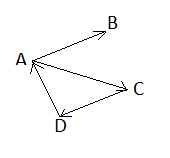
\includegraphics[scale=1]{images/17_oriente.png}
\caption{Graphe orienté}
\end{figure}
\item \textbf{Les graphes non orientés} (sans flèche, sans direction). Une arête est un ensemble de deux nœuds. On ne parle pas de "paire" vu que l'ordre des nœuds n'a pas d'importance. Ici, parler de l'arête (A,B) ou (B,A) revient à la même chose.
\begin{figure}[!h]
\centering
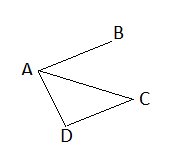
\includegraphics[scale=1]{images/17_non-oriente.png}
\caption{Graphe non orienté}
\end{figure}
\\
\end{itemize}
Dans le cours, on aura surtout affaire à des graphes non orientés.

\paragraph{Notions de chemins et de connectivité}
\begin{itemize}

\item \textbf{Chemin} : séquence (un ordre) de nœud. Chaque paire consécutive est une arête. Un chemin peut passer plusieurs fois par la même arête (boucle), ce qui n'est pas toujours ce qu'on veut.
\item \textbf{Chemin simple} : chaque nœud est au maximum une fois dans la séquence. On ne peut plus faire le tour plusieurs fois.
\item \textbf{Cycle} : chemin qui arrive au même endroit d'où il est parti. 
	\begin{itemize}
			
	\item Le premier et le dernier nœud sont les mêmes. 
	\item Le chemin a au moins 3 liens (puisqu'on ne peut pas passer plusieurs fois par la même 	arête). 

\end{itemize}
\end{itemize}